\documentclass[../../main]{subfiles}
\begin{document}

\subsection{Overall system architecture}
\label{ss:overall-system-architecture}

The proposed system is composed by two main parts:
\begin{itemize}
    \item a \textbf{mobile application}, acting as the client with which users can interact with the system itself;
    \item a \textbf{backend server}, that receives incoming requests from the clients and handles them.
\end{itemize}
Other than these two, our system also requires:
\begin{itemize}
    \item an \textbf{authentication service}, a way for allowing users to be authenticated and collect data linked to them;
    \item a \textbf{push notification service}, for contacting the users even without direct request from them.
\end{itemize}
An overall diagram describing the architecture follows.
\begin{figure}[h]
    \centering
    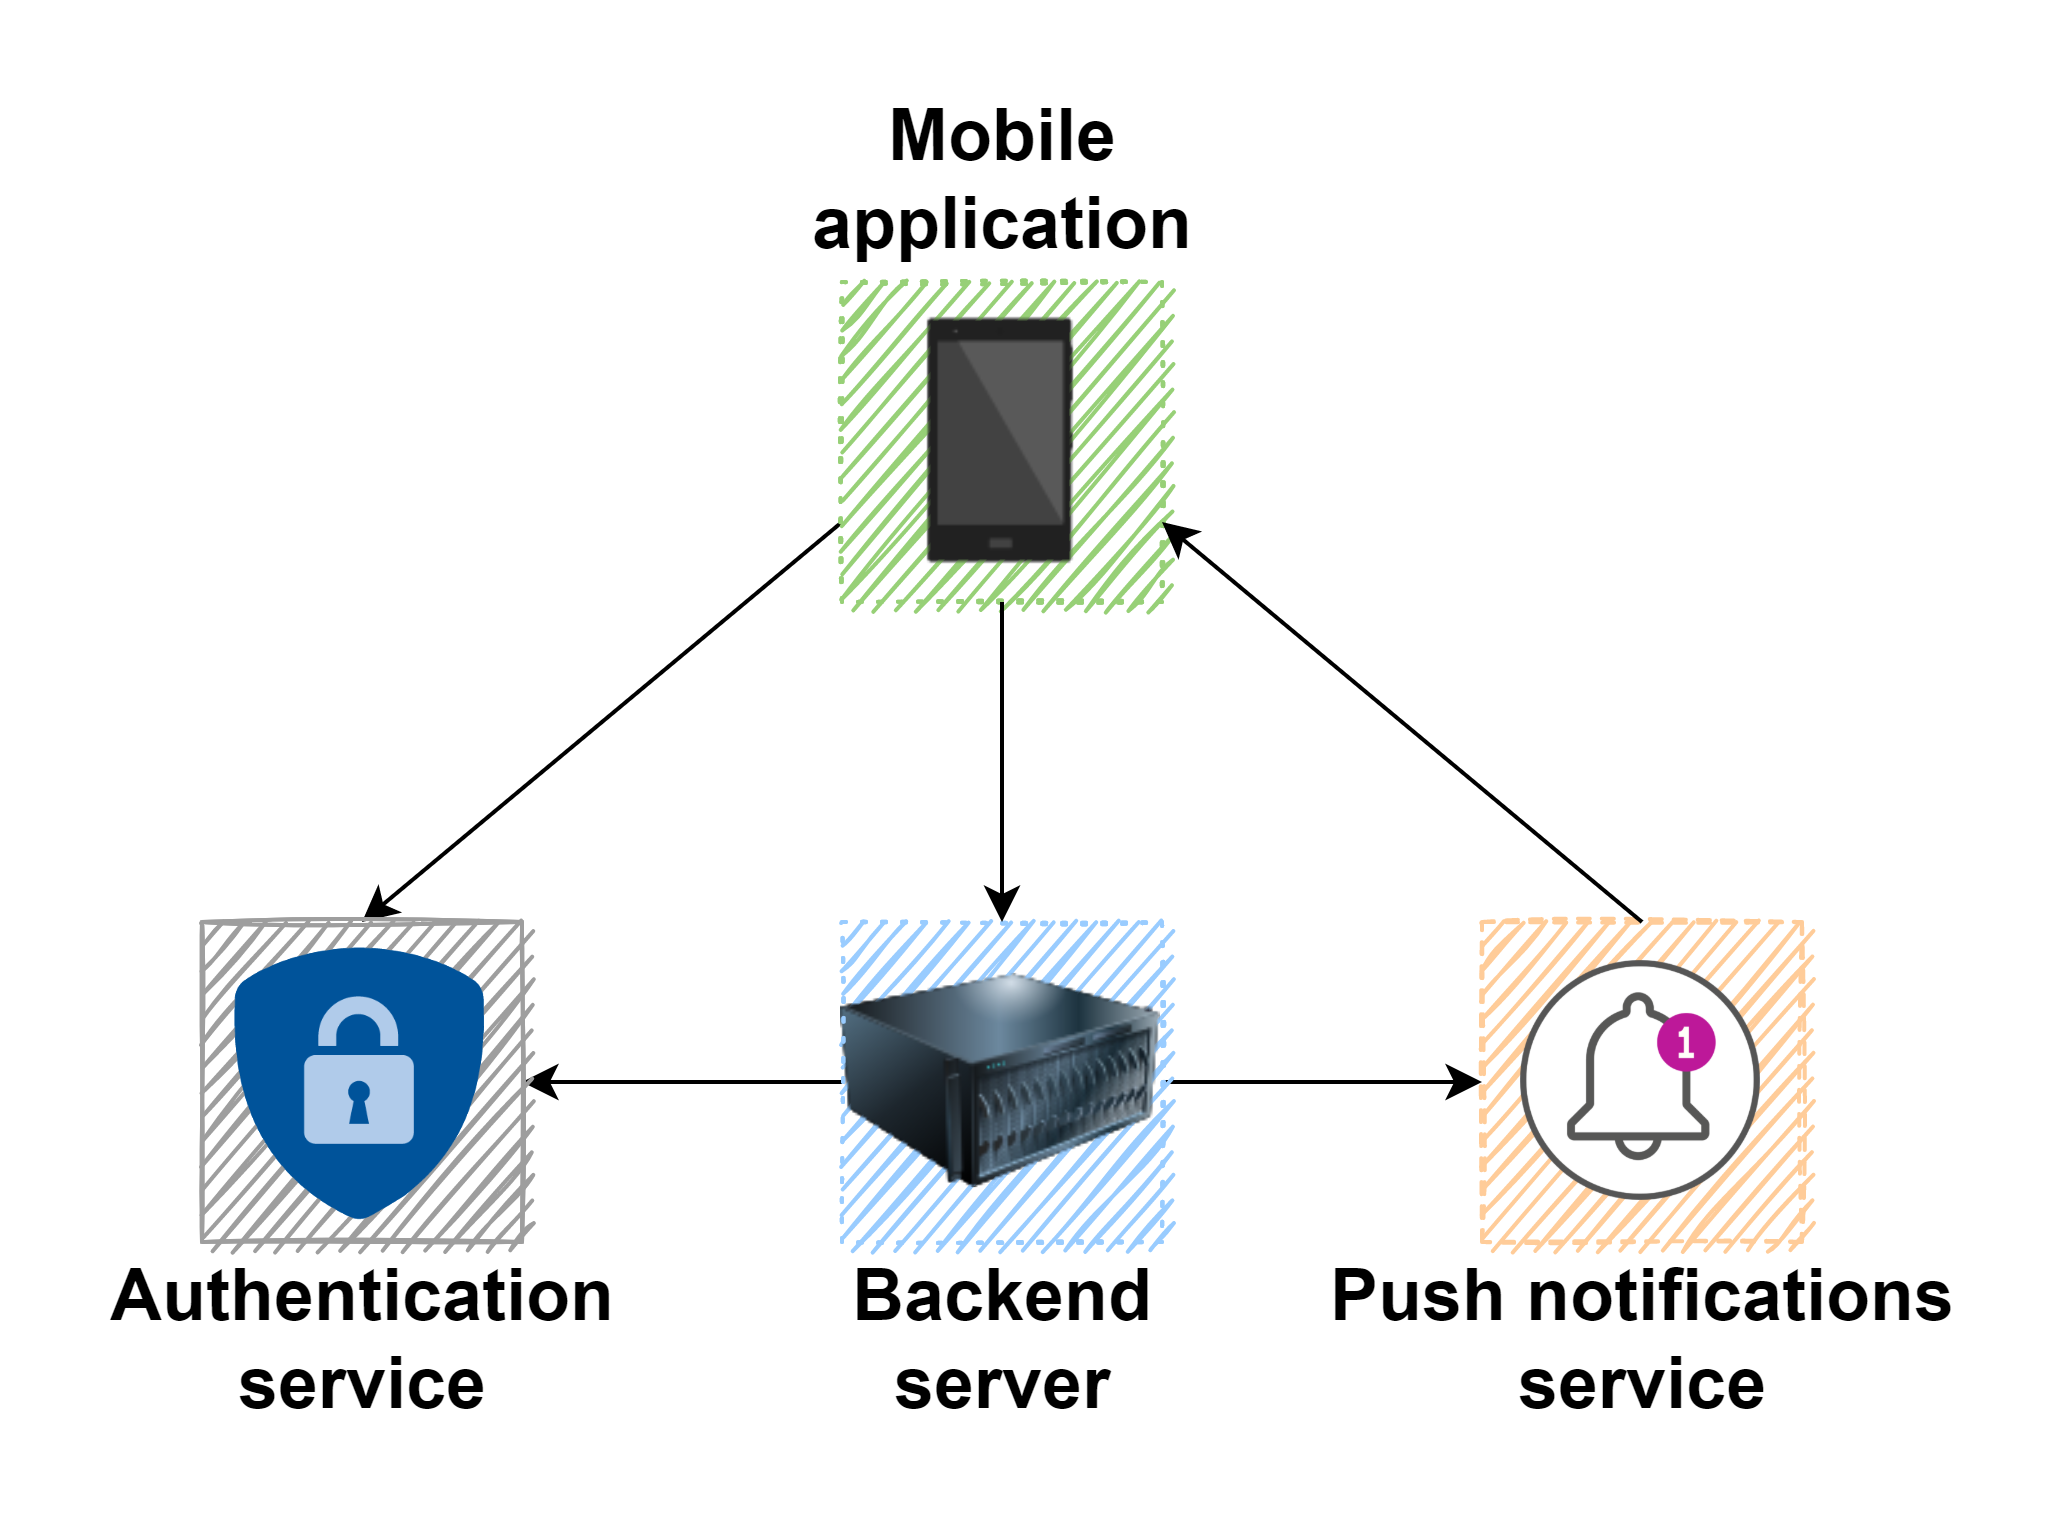
\includegraphics[width=0.7\textwidth]{images/overall_system_architecture}
    \caption{Overall system architecture}\label{fig:overall_system_architecture}
\end{figure}

\noindent
We will go more in detail about the \textbf{mobile application} and the \textbf{backend server} in the following two sections; here we just want to discuss a little more about the \textbf{authentication} and \textbf{push notification} \textbf{services}.
\newpage
\subsubsection{Authentication service}
Since the goal of the project was to develop a context-aware system, we chose to focus on this aspect and try to take advantage of already available software.\\
In the area of authentication, there are many providers that offer this kind of service.\\
Our need is that this kind of service allows users to:
\begin{itemize}
    \item register an account with an e-mail address and a password;
    \item login with the credentials they used for registering;
    \item generate temporary tokens that have their correctness verifiable by the service itself, so to allow users to use them for showing they were granted access to the system.
\end{itemize}

\subsubsection{Push notification service}
For the two main mobile operating systems, Android and iOS, there are already technologies that enable this requirement in a way that suit our needs.
In this situation, it would be really reinventing the wheel trying to implement this service ourselves and therefore we just need a service that allows to:
\begin{itemize}
    \item send notifications at every time of the day to users that have registered for receiving them;
    \item it is not specific to an operating system only.
\end{itemize}

\end{document}